% ============================================================
%  Piezoelectric Actuator Preload Diagrams
%  Figure 1: Mass Preload
%  Figure 2: Spring Preload
%
%  Compile with: pdflatex piezo_preload_diagrams.tex
%  Requires: tikz, decorations.pathmorphing library
% ============================================================

\documentclass[border=6pt]{standalone}
\usepackage{tikz}
\usetikzlibrary{
	patterns,
	arrows.meta,
	decorations.pathmorphing,
	decorations.pathreplacing,
	calc
}
\usepackage{amsmath}

% ---- Colour palette ----------------------------------------
\colorlet{PGreen}{green!55!black}   % piezo A (green)
\colorlet{PRed}{red!65!black}       % piezo B (red)
\colorlet{LBlue}{cyan!55!blue}      % load line / operating region

% ---- Reusable: striped piezo block -------------------------
%  #1 x-left  #2 y-bottom  #3 x-right  #4 y-top  #5 color
\newcommand{\piezoblock}[5]{%
	\begin{scope}
		\clip (#1,#2) rectangle (#3,#4);
		\foreach \ii in {0,...,22}{%
			\fill[#5!72] (#1,{#2+\ii*0.205}) rectangle (#3,{#2+\ii*0.205+0.135});
		}
	\end{scope}
	\draw[thick] (#1,#2) rectangle (#3,#4);
}

% ---- Reusable: floor-ground symbol -------------------------
%  #1 x-centre  #2 y-line  #3 half-width
\newcommand{\gnd}[3]{%
	\draw[thick] ({#1-#3},#2) -- ({#1+#3},#2);
	\fill[pattern=north east lines, pattern color=black!55]
	({#1-#3},{#2-0.28}) rectangle ({#1+#3},#2);
}

% ---- Reusable: ceiling-mount symbol (hatching above line) --
%  #1 x-left  #2 x-right  #3 y-line
\newcommand{\ceiling}[3]{%
	\draw[thick] (#1,#3) -- (#2,#3);
	\fill[pattern=north east lines, pattern color=black!55]
	(#1,#3) rectangle (#2,{#3+0.28});
}

% ---- Reusable: vertical coil spring ------------------------
%  #1 x  #2 y-start  #3 x (same)  #4 y-end
\newcommand{\springV}[4]{%
	\draw[thick,
	decoration={coil, aspect=0.38, segment length=3.5pt, amplitude=4.5pt},
	decorate] (#1,#2) -- (#3,#4);
}

% ---- Shared hysteresis loop A (green, wider band) ----------
%  #1=x-graph-origin  #2=y-graph-origin
\newcommand{\loopA}[2]{%
	\fill[PGreen!28]
	({#1+0.15},{#2+0.10})
	.. controls ({#1+1.25},{#2+0.98}) and ({#1+2.35},{#2+2.05}) ..
	({#1+3.15},{#2+3.13})
	.. controls ({#1+2.72},{#2+2.90}) and ({#1+1.72},{#2+1.82}) ..
	({#1+0.00},{#2+0.06}) -- cycle;
	\draw[PGreen!85!black, line width=1.4pt]
	({#1+0.15},{#2+0.10})
	.. controls ({#1+1.25},{#2+0.98}) and ({#1+2.35},{#2+2.05}) ..
	({#1+3.15},{#2+3.13});
	\draw[PGreen!85!black, line width=1.4pt]
	({#1+0.00},{#2+0.06})
	.. controls ({#1+1.72},{#2+1.82}) and ({#1+2.72},{#2+2.90}) ..
	({#1+3.15},{#2+3.13});
	\node[PGreen!78!black, font=\bfseries] at ({#1+1.35},{#2+2.78}) {A};
}

% ---- Shared hysteresis loop B (red, narrower band) ---------
%  #1=x-graph-origin  #2=y-graph-origin
\newcommand{\loopB}[2]{%
	\fill[PRed!28]
	({#1+0.08},{#2+0.04})
	.. controls ({#1+1.10},{#2+0.55}) and ({#1+2.35},{#2+1.65}) ..
	({#1+3.20},{#2+2.30})
	.. controls ({#1+2.10},{#2+1.98}) and ({#1+0.72},{#2+0.82}) ..
	({#1+0.08},{#2+0.04}) -- cycle;
	\draw[PRed!85!black, line width=1.4pt]
	({#1+0.08},{#2+0.04})
	.. controls ({#1+1.10},{#2+0.55}) and ({#1+2.35},{#2+1.65}) ..
	({#1+3.20},{#2+2.30});
	\draw[PRed!85!black, line width=1.4pt]
	({#1+0.08},{#2+0.04})
	.. controls ({#1+0.72},{#2+0.82}) and ({#1+2.10},{#2+1.98}) ..
	({#1+3.20},{#2+2.30});
	\node[PRed!85!black, font=\bfseries] at ({#1+2.45},{#2+1.60}) {B};
}

\newcommand{\loopC}[2]{%
	\fill[PRed!28]
	({#1+0.15},{#2+0.10})
	.. controls ({#1+1.25},{#2+0.98}) and ({#1+2.35},{#2+2.05}) ..
	({#1+3.15},{#2+3.13})
	.. controls ({#1+2.72},{#2+2.90}) and ({#1+1.72},{#2+1.82}) ..
	({#1+0.00},{#2+0.06}) -- cycle;
	\draw[PRed!85!black, line width=1.4pt]
	({#1+0.15},{#2+0.10})
	.. controls ({#1+1.25},{#2+0.98}) and ({#1+2.35},{#2+2.05}) ..
	({#1+3.15},{#2+3.13});
	\draw[PRed!85!black, line width=1.4pt]
	({#1+0.00},{#2+0.06})
	.. controls ({#1+1.72},{#2+1.82}) and ({#1+2.72},{#2+2.90}) ..
	({#1+3.15},{#2+3.13});
	\node[PRed!78!black, font=\bfseries] at ({#1+1.35},{#2+2.58}) {B};
}

% ============================================================
\begin{document}

	
	%% ===========================================================
	%%  FIGURE 2 -- Spring Preload
	%% ===========================================================
	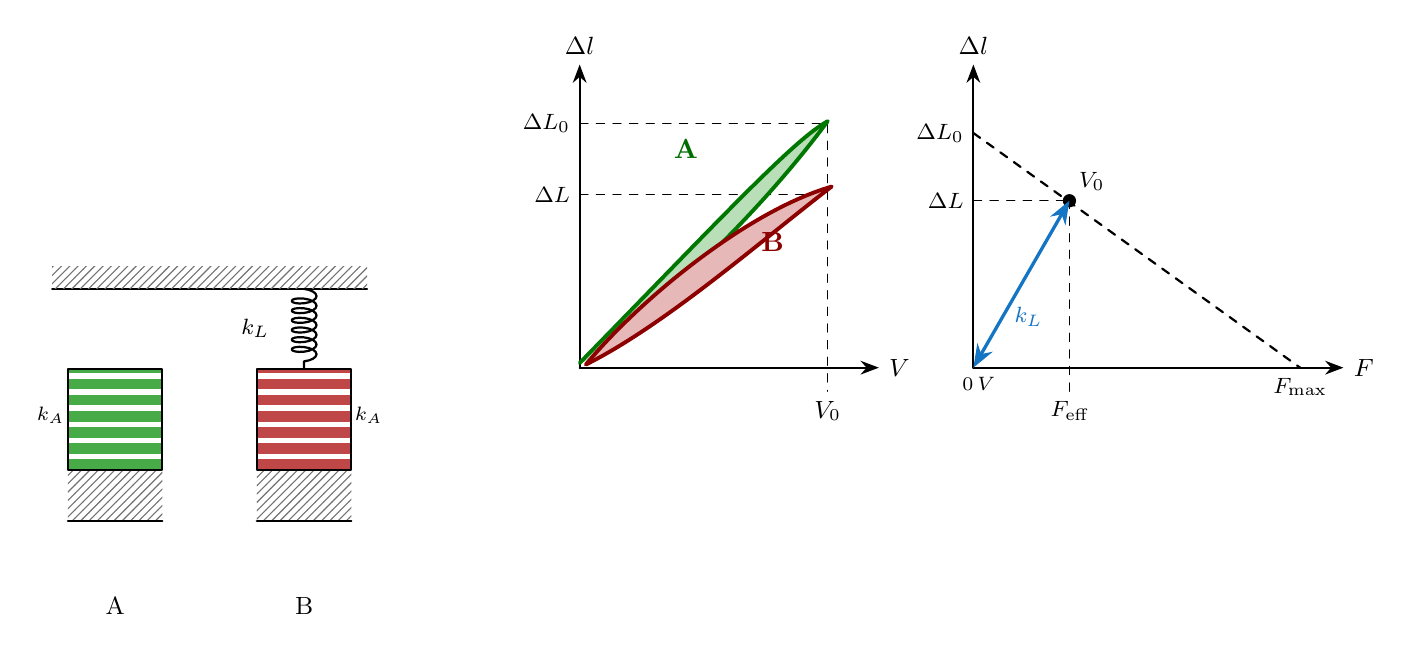
\begin{tikzpicture}[font=\small, >=Stealth, line cap=round, line join=round]
		
		% -- Ceiling for spring kL -----------------------------------
		\ceiling{-6.0}{-2.0}{2.3}
		
		% -- Spring kL (vertical, centred) ---------------------------
		\springV{-2.8}{2.3}{-2.8}{1.30}
		\node[right,font=\footnotesize] at (-3.72,1.80) {$k_L$};
		
		% -- Actuator A (green) with kA spring below -----------------
		\fill[pattern=north east lines, pattern color=black!55]
		(-5.80,-.65) rectangle (-4.60,0);
		\draw[thick] (-5.80,-0.65) -- (-4.60,-0.65);
		\node[left,font=\scriptsize] at (-5.72,.7) {$k_A$};
		\piezoblock{-5.80}{0}{-4.60}{1.28}{PGreen}
		\node[below=24pt] at (-5.20,-0.65) {A};
		
		% -- Actuator B (red) with kA spring below -------------------
		\fill[pattern=north east lines, pattern color=black!55]
		(-3.40,-.65) rectangle (-2.20,0);
		\draw[thick] (-3.40,-0.65) -- (-2.20,-0.65);
		\node[right,font=\scriptsize] at (-2.28,.7) {$k_A$};
		\piezoblock{-3.40}{0}{-2.20}{1.28}{PRed}
		\node[below=24pt] at (-2.80,-0.65) {B};
		
		% -- Center: DeltaL vs V (with DeltaL operating level) -------
		\def\Gox{0.7}
		
		\draw[->,thick] (\Gox,1.3) -- ({(\Gox)+3.8},1.3) node[right] {$V$};
		\draw[->,thick] (\Gox,1.3) -- (\Gox,1.3+3.85)       node[above] {$\Delta l$};
		
		\draw[dashed,thin]
		(\Gox,4.4) -- ({(\Gox)+3.15},4.4) -- ({(\Gox)+3.15},1)
		node[below] {$V_0$};
		\node[left,font=\footnotesize] at (\Gox,4.4) {$\Delta L_0$};
		
		% DeltaL operating level
		\draw[dashed,thin]
		(\Gox,3.5) -- ({(\Gox)+3.15},3.5);
		\node[left,font=\footnotesize] at (\Gox,3.5) {$\Delta L$};
		
		\loopA{\Gox}{1.3}
		\loopB{\Gox}{1.3}
		
		% -- Right: DeltaL vs F (spring preload) ---------------------
		\def\Fox{5.7}
		
		\draw[->,thick] (\Fox,1.3) -- ({(\Fox)+4.7},1.3) node[right] {$F$};
		\draw[->,thick] (\Fox,1.3) -- (\Fox,3.85+1.3)       node[above] {$\Delta l$};
		
		\node[left,font=\footnotesize] at (\Fox,4.28) {$\Delta L_0$};
		
		% Dashed free-stroke line at V0
		\draw[dashed,thick]
		(\Fox,4.28) -- ({(\Fox)+4.15},1.3)
		node[below,font=\footnotesize] {$F_{\max}$};
		
		% Operating point (spring load line meets free-stroke line at V0)
		\coordinate (OP) at ({(\Fox)+1.22},3.42);
		\fill (OP) circle (2.4pt);
		\node[above right,font=\footnotesize] at (OP) {$V_0$};
		
		% DeltaL horizontal dashed
		\draw[dashed,thin]
		(\Fox,3.42) node[left,font=\footnotesize]{$\Delta L$} -- (OP);
		
		% Feff vertical dashed
		\draw[dashed,thin]
		({(\Fox)+1.22},1) node[below,font=\footnotesize]{$F_{\text{eff}}$} -- (OP);
		
		% Blue spring load line kL (origin -> operating point, with arrow)
		\draw[LBlue, very thick, <->] (\Fox,1.3) -- (OP);
		\node[LBlue, font=\footnotesize] at ({(\Fox)+0.70},1.95) {$k_L$};
		
		% 0V at graph origin
		\node[below left,font=\scriptsize] at (\Fox+.4,1.3) {$0\,V$};
		
	\end{tikzpicture}
	
\end{document}